% 2017 浙江 21 图：抛物线 x^2=y；A(-1/2,1/4)，B(3/2,9/4)，P 为抛物线上动点（取 k=1/4 代表位置），Q 为 B 到 AP 的垂足。
% 全局数值坐标，单位比率 1.5cm，线宽 .6pt，12pt。
\usetikzlibrary{arrows.meta,calc}
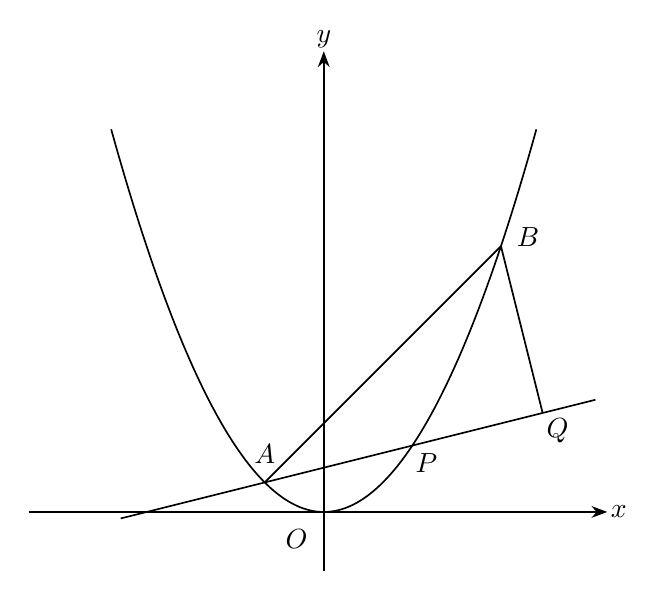
\begin{tikzpicture}[x=1.5cm,y=1.5cm,line width=.6pt,>=Stealth,font=\normalsize]
\coordinate (O) at (0,0);
\coordinate (A) at (-0.5,0.25);
\coordinate (B) at (1.5,2.25);
\coordinate (P) at (0.75,0.5625);
\coordinate (Q) at (1.852941,0.838235);
\draw[->] (-2.5,0)--(2.4,0) node[right,inner sep=1pt] {$x$};
\draw[->] (0,-0.5)--(0,3.9) node[above,inner sep=1pt] {$y$};
\draw[domain=-1.8:1.8,samples=121] plot (\x,{\x*\x});
\draw (-1.72,-0.055)--(2.30,0.95);
\draw (A)--(B);
\draw (B)--(Q);
\node[inner sep=1pt] at (-0.5,0.49) {$A$};
\node[inner sep=1pt] at (1.73,2.33) {$B$};
\node[inner sep=1pt] at (0.87,0.41) {$P$};
\node[inner sep=1pt] at (1.98,0.69) {$Q$};
\node[inner sep=1pt] at (-0.23,-0.23) {$O$};
\end{tikzpicture}
